\chapter{Formale Sprachen}
\index{Formale Sprachen}
%
Die Informatik macht sich Gedanken um die systematische Verarbeitung von Information. Anhand verschiedener Modelle haben wir bereits gesehen, wie wir eine Eingabe nehmen, diese nach Vorschriftsregeln verarbeiten und dann eine Antwort auf das gestellte Anfangsproblem liefern. Dabei haben wir eine wichtige Frage wegfallen lassen: Woher weiß der Algorithmus, ob diese Eingabe valid ist? Woher weiß die Turingmaschine, dass das (was auf dem Band steht) eine korrekte Eingabe ist, die zu keinem undefinierten Verhalten führt?\footnote{Als Beispiel für undefiniertes Verhalten sei hier die Division durch Null gegeben.}

\index{Wortproblem}
Das Wortproblem stellt folgende Frage:
\begin{quotation}
  Gegeben sei eine Sprache $S$. Ermittle, ob ein Wort $W$ Teil von $S$ ist oder nicht.
\end{quotation}
%
Wir verwenden die neuen Begriffe \emph{Wort} (oder String bzw. Zeichenkette) und \emph{Sprache} (Vorschriften über die mögliche Aneinanderreihung von Wörtern). Eine Sprache beschreibt eine Menge von Wörtern\footnote{Beachte, dass Wort anders als im linguistischen Sinn betrachtet wird. So ist ein Satz wie ,,Der Gärtner ist der Mörder`` \emph{ein} Wort einer Sprache.}. Für diese muss eine Zugehörigkeitsbeziehung ermittelt werden können. Wir führen das Konzept der Sprachen und Grammatiken ein.

\section{Eine einfache Sprache}
\index{Reguläre Ausdrücke!Beispiel}
%
Gegeben sei eine einfache Sprache $S$, die genau nur 1 Zeichenkette akzeptieren soll und zwar jene, die nur aus \gramm{a} besteht. Stimmt das Eingabewort $W$ mit der Zeichenkette \gramm{a} überein, wird die Eingabe akzeptiert; andernfalls zurückgewiesen. So wird das Wortproblem entschieden. Da wir die Sprache als Menge repräsentieren können, verwenden wir Mengennotation: $S = \{\texttt{a}\}$ und das Wortproblem für einen String $s$ lautet $s \stackrel{?}{\in} S$.
%
\begin{figure}[ht]
 \begin{center}
  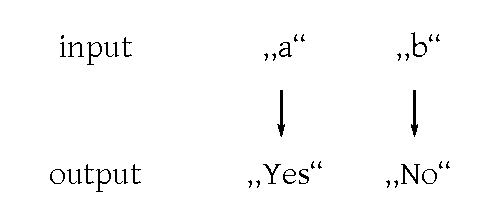
\includegraphics{img/wordproblem.pdf}
  \caption{Zwei Beispiele für die Entscheidung das Wortproblems für die Sprache \gramm{a}.}
  \label{fig:wordproblem}
 \end{center}
\end{figure}

Ein komplexeres Beispiel verwendet mehrere Zeichen: Die Sprache $T$ als \gramm{abb} akzeptiert genau jene Wörter, die eine Länge 3 und den Aufbau ,,abb`` haben.

Wir möchten in diesem Kapitel also Sprachen definieren. Wir haben eine textuelle Beschreibung verwendet. Wir haben auch Mengennotation verwendet. Wobei diese Ansätze durchaus legitim sind, besitzt der textuelle Ansatz das Problem fehleranfällig zu sein (Spezialfälle werden nicht spezifiziert) und Mengennotation kann komplexere Sprachen nicht übersichtlich abbilden. Wir befassen uns daher mit zwei weiteren Ansätzen in den folgenden Abschnitten:
\index{Reguläre Ausdrücke}
\begin{itemize}
  \item reguläre Ausdrücke (kompakte Schreibweise für eine bestimmte Untermenge von Sprachen)
  \item formale Grammatiken (ein mächtiges Werkzeug um allgemeine Grammatiken zu beschreiben)
\end{itemize}

\subsubsection*{Unsere einfachen Sprachen in Mengennotation}
\index{Reguläre Ausdrücke!Beispiel}
\index{Formale Grammatiken!Beispiel}
\[
  S = \{\texttt{a}\}  \qquad  T = \{\texttt{abb}\}
\]

\subsubsection*{Unsere einfachen Sprachen als regulärer Ausdruck}
\lstset{language={}, label={lst:regex_S}, caption={$S$ als regulärer Ausdruck}, frame={single}}
\begin{lstlisting}
a
\end{lstlisting}
\lstset{language={}, label={lst:regex_T}, caption={$T$ als regulärer Ausdruck}, frame={single}}
\begin{lstlisting}
abb
\end{lstlisting}

\subsubsection*{Unsere einfachen Sprachen als formale Grammatik}
\lstset{language={}, label={lst:regex_S}, caption={$S$ als formale Grammatik $G=(V,\Sigma,P,S)$}, frame={single}, escapechar=\@}
\begin{lstlisting}
S @$\rightarrow$@ a
\end{lstlisting}
\lstset{language={}, label={lst:regex_T}, caption={$T$ als formale Grammatik $G=(V,\Sigma,P,S)$}, frame={single}, escapechar=\@}
\begin{lstlisting}
S @$\rightarrow$@ abb
\end{lstlisting}

\section{Eine Sprache mit Wiederholungen}
%
Wir möchten unsere Sprachendefinitionen erweitern, indem wir eine Anzahl abbilden können. So war es uns bislang nicht möglich eine Sprache (zB) ,,Akzeptiere alle Wörter die nur aus \emph{a}s bestehen`` zu formulieren. Hierfür müssen wir Wiederholungen repräsentieren.

\subsection{In regulären Ausdrücken}
\index{Reguläre Ausdrücke!Quantoren}
%
Wir führen das Konzept der Quantoren ein. Ein regulärer Ausdruck ist eine Zeichenkette, die ein oder mehrere Zeichenketten spezifiziert. Grundsätzlich wird für reguläre Ausdrücke jenes Wort notiert, welches innerhalb der Sprache liegt. Wir lernen jetzt Konzepte kennen, um mehrere Wörter abzubilden.
%
\begin{table}[ht]
 \begin{center}
  \begin{tabular}{cl}
   \hline
    \texttt{+} & Das vorige Zeichen kommt 1--$\infty$ mal vor (,,1-mal oder öfters``) \\
    \texttt{*} & Das vorige Zeichen kommt 0--$\infty$ mal vor (,,beliebig oft``) \\
    \texttt{?} & Das vorige Zeichen kommt 0--1 mal vor (,,optional``) \\
   \hline
  \end{tabular}
  \caption{Quantoren in regulären Ausdrücken}
  \label{tab:quantifiers}
 \end{center}
\end{table}

\index{Quantoren (reguläre Ausdrücke)}
In Tabelle~\ref{tab:quantifiers} werden Quantoren definiert. Kommen diese Zeichen in einem regulären Ausdruck vor, werden diese nicht wortwörtlich verstanden, sondern beziehen sich auf das letzte Zeichen oder die letzte Gruppe.

Wir betrachten ein Beispiel. Gesucht sei folgende Sprache $R$:
\begin{quote}
  Das Zeichen \gramm{a} kann (aber muss nicht) vorkommen. Nachfolgend kommt ein \gramm{b} und
  anschließend beliebig viele \gramm{c}.
\end{quote}

Der folgende Ausdruck spezifiziert diese Sprache:
\lstset{language={}, label={lst:regex_repetition}, caption={Die Sprache~$R$ als regulärer Ausdruck}, frame={single}}
\begin{lstlisting}
a?bc*
\end{lstlisting}

Das erste Fragezeichen bezieht sich auf das vorige Zeichen ,,a`` und macht es optional. Das folgende ,,b`` muss zwingend vorkommen. Dem ,,c`` ist ein Stern nachgestellt und ein Stern spezifiziert die Quantität ,,beliebig oft``.

\subsection{In Mengennotation}
%
In Mengennotation wird $R$ als $\{a^n b c^m | 0\leq n\leq 1, m \geq 0\}$ notiert. Hierbei wird die Anzahl der Vorkommnisse eines Zeichens oder einer Gruppe mit einer hochgestellten Zahl notiert. Wird die Domäne der Variable ($n$ und $m$) nicht angegeben, spricht man von natürlichen Zahlen inklusive der 0.

\subsection{Als formale Grammatik}
\index{Reguläre Ausdrücke!Beispiel}
\index{Formale Grammatiken!Beispiel}
%
In einer formalen Grammatik ist Wiederholung über Rekursion abzubilden.

Aber besprechen wir zuerst, was formale Grammatiken denn sind und wie sie Wörter erzeugen. Eine formale Grammatik $G = (V, \Sigma, P, S)$ besitzt ein endliches Vokabular $V$, ein Alphabet $\Sigma$, Produktionsregeln $P$ und ein Startsymbol $S$. Das Erzeugen von Strings startet stets mit dem Startsymbol $S$ und Produktionsregeln $P$ erlauben es uns Zeichen sukzessive durch Zeichen aus $V$ zu ersetzen. Wir unterscheiden dabei zwischen den Terminalsymbolen $\Sigma$ und Nonterminalsymbolen $V \setminus \Sigma$. Terminalsymbole sind jene Symbole, die in der endgültigen Zeichenkette vorkommen. Für Nonterminalsymbole sind Regeln in $P$ definiert, wie man sie ersetzen kann. Die Ersetzungen erfolgen so lange bis nur mehr Terminalsymbole enthalten sind.

% TODO: ,` and ,,`` in wrong order
Als ersten Schritt (um $R$ zu definieren) beschreiben wir eine Sprache~$R1$ mit ,Das Zeichen \gramm{a} kann vorkommen`.
\lstset{language={}, label={lst:regex_R1}, caption={$R1$ als formale Grammatik $G=(V,\Sigma,P,S)$}, frame={single}, escapechar=\@}
\begin{lstlisting}
S @$\rightarrow$@ a
S @$\rightarrow$@
\end{lstlisting}

Wir starten also mit einem Startsymbol ,,S`` und ersetzen es jetzt. Entweder wir entscheiden uns für die Zeile 1 und setzen ,,a`` ein oder einen leeren String ,,`` (Zeile 2).

Als zweiten Schritt beschreiben wir eine Grammatik $R2$ mit ,Das Zeichen \gramm{a} kann vorkommen. Nachfolgend kommt ein \gramm{b}`.
\lstset{language={}, label={lst:regex_R2}, caption={$R2$ als formale Grammatik $G=(V,\Sigma,P,S)$}, frame={single}, escapechar=\@}
\begin{lstlisting}
S @$\rightarrow$@ ab
S @$\rightarrow$@ b
\end{lstlisting}

Nachdem ein optionales \texttt{a} angegeben wurde, folgt ein \texttt{b}. Für die Wiederholung von \texttt{c} verwenden wir ein Nonterminalsymbol \texttt{T} (welches per Konvention großgeschrieben wird).
\lstset{language={}, label={lst:regex_R3}, caption={$R$ als formale Grammatik $G=(V,\Sigma,P,S)$}, frame={single}, escapechar=\@}
\begin{lstlisting}
S @$\rightarrow$@ abT
S @$\rightarrow$@ bT
T @$\rightarrow$@
T @$\rightarrow$@ cT
\end{lstlisting}

Gehen wir die Produktionsregeln für den Eingabestring \texttt{abcc} durch. Wir starten wieder mit dem Startsymbol ,,S``. Wir ersetzen es mittels der 1. Zeile zu ,,abT``. Wir erkennen ein verbleibendes Nonterminal in ,,T`` in dem String und suchen uns hierfür entsprechende Regeln; die Regeln 3 und 4 kommen in Frage. Für den gegebenen Eingabestring müssen wir Regel 4 verwenden. Es entsteht der String ,,abcT``. Wieder ersetzen wir das ,,T`` durch die Regel 4. ,,abcT`` besitzt auch noch ein Nonterminal, welches jetzt jedoch mittels Regel 3 ersetzt wird. Es entsteht der String ,,abcc`` (bestehend nur aus Terminalsymbolen). Damit liegt der String ,,abcc`` in der durch die formale Grammatik spezifizierten Sprache.

\section{Alternation in Sprachen}
%
Gesucht sei folgende Sprache~$A$:
\begin{quote}
  Die Zeichenkette beginnt mit ,,message of the `` und endet entweder mit ,,day`` oder ,,week``. Am Ende befindet sich weiters ein Rufzeichen ,,{!}``.
\end{quote}

\subsection{Als regulärer Ausdruck}
\index{Reguläre Ausdrücke!Beispiel}
%
In einem regulären Ausdruck lässt sich eine Alternation definieren, indem der vertikale Balken als Alternationsoperator verwendet wird. Dabei wird entweder die linke Seite vom Balken oder die rechte Seite herangezogen. Die Seiten können durch eine Gruppierung beschränkt werden, die durch runde Klammern definiert wird.

\lstset{language={}, label={lst:regex_alternation}, caption={Die Sprache $A$}, frame={single}}
\begin{lstlisting}
message of the (day|week)!
\end{lstlisting}

\subsection{Als formale Grammatik}
\index{Formale Grammatiken!Beispiel}
%
Alternation haben wir schon implizit bei formalen Grammatiken kennen gelernt. Wir wählen aus mit welcher Regel wir ein Nonterminalsymbol ersetzen.
%
\lstset{language={}, label={lst:regex_A}, caption={$A$ als formale Grammatik $G=(V,\Sigma,P,S)$}, frame={single}, escapechar=\@}
\begin{lstlisting}
S @$\rightarrow$@ message of the T!
T @$\rightarrow$@ day
T @$\rightarrow$@ week
\end{lstlisting}

Wir haben jetzt die wichtigsten Konzepte betrachtet, um Sprachen definieren zu können. Wir möchten jetzt noch auf ein paar spezifische Details eingehen und die Mächtigkeit von Sprachen evaluieren.

\section{Reguläre Ausdrücke}
\index{Reguläre Ausdrücke!Operatoren}
%
\begin{table}[ht]
 \begin{center}
  \begin{tabular}{cl}
   \hline
    \texttt{.}     & Ein beliebiges Zeichen (aus $\Sigma$) \\
    \texttt{[ab]}  & Eines der Zeichen aus $\set{\texttt{a}, \texttt{b}}$ (Zeichenmenge) \\
    \texttt{(ab)}  & Fasst die Sequenz ,,ab`` zu einer Gruppe zusammen (Gruppierung) \\
    \texttt{a|bc}  & Entweder ,,a`` oder ,,bc`` (Alternation) \\
    \texttt{+}     & Das vorige Zeichen kommt 1--$\infty$ mal vor (,,1-mal oder öfters``) \\
    \texttt{*}     & Das vorige Zeichen kommt 0--$\infty$ mal vor (,,beliebig oft``) \\
    \texttt{?}     & Das vorige Zeichen kommt 0--1 mal vor (,,optional``) \\
   \hline
  \end{tabular}
  \caption{RegEx Operatoren}
  \label{tab:regex_op}
 \end{center}
\end{table}
%
Reguläre Ausdrücke (engl. ,,regular expressions`` oder kurz RegEx) sind eine kompakte Schreibweise, um mehrere Zeichenketten darzustellen. In Tabelle~\ref{tab:regex_op} sind die Sonderzeichen nochmals zusammengefasst dargestellt. In der Tabelle wird eine Möglichkeit genannt eine Zeichenmenge anzugeben. Dieses Konzept kann genauso durch eine Alternation simuliert werden.

\subsection{Non-greedy Verhalten}
\index{Greediness (Reguläre Ausdrücke)}
%
RegEx-Implementierungen gibt es unterschiedliche. Die zwei großen Implementierungen nennen sich ,,POSIX`` und ,,PCRE``. Diese unterscheiden sich durch ihren Aufbau und ihre erweiterten Möglichkeiten. Ich möchte hier auf ein Detail eingehen.

Eine häufig vorkommende Struktur bei regulären Ausdrücken ist \texttt{(.*)}. Es handelt es sich um eine Gruppe von beliebigen Zeichen beliebiger Länge. Salopp gesprochen matcht dieser Ausdruck jeden String.
Wie sieht es nun mit dem regulären Ausdruck \texttt{(.*)} und der Eingabe ,,abc`` aus? Greedy-Verhalten bezeichnet das Bestreben eines Ausdrucks, möglichst viel Inhalt zu matchen. Entsprechend würde dieser Ausdruck die gesamte Eingabe matchen, da sie versucht sich alles zuzuweisen. Dies verwirrt viele RegEx-Benutzer, da ein RegEx \texttt{a(.*)a} bei dem Eingabestring ,,abaaba`` nicht ,,aba`` zweimal matcht, sondern einmal ,,abaaba``. RegEx sind für gewöhnlich immer bestrebt möglichst viel zu matchen.

Non-greedy Verhalten kann man durch das Anfügen eines Fragezeichens nach dem Gruppenquantor erreichen; ist allerdings nur bei ,,PCRE``-Engines verfügbar. Für unser Beispiel wäre etwa \texttt{a(.*?)a} sinnvoll um den String in zwei Teilen zu matchen.

\subsection{Deterministische Automaten}
\index{Konvertierung!von regulären Ausdrücken zu Automaten}
%
Abseits der Strings mit den jeweiligen Operatoren gibt es auch eine andere Darstellungsweise für reguläre Ausdrücke. Zu jedem regulären Ausdruck kann ein deterministischer Automat gefunden. Ein deterministischer Automat ist ein gerichteter, kantenbeschrifteter Graph. Wir erinnern uns, dass ein Graph aus Knoten und Kanten besteht. Es gibt einen Startknoten\footnote{In diesem Dokument folgen wir der Konvention, dass der Startknoten der am weitesten links positionierte Knoten ist. Im Allgemeinen handelt es sich um den einzigen Quellknoten im Graphen.} und von diesem ausgehend werden die Zeichen vom Eingabestring gelesen. Je nach gelesenem Zeichen folgt man jenen Kanten, deren Beschriftung mit dem Zeichen übereinstimmt. Ein Eingabestring wird genau dann von der Sprache akzeptiert, wenn der String auf einem Endknoten zu Ende geht, der durch einen zusätzlichen inneren Kreis markiert ist.

\index{Nichtdeterminismus!Automaten von regulären Sprachen}
Das Wesentliche ist, dass dieser Automat das Kriterium des Determinismus zu erfüllen hat. Dies bedeutet in jedem beliebigen Zustand des Automaten kann durch das gelesene Zeichen eindeutig bestimmt werden welcher Kante zu folgen ist. Oder in anderen Worten gibt es keine zwei Kanten mit der selben Beschriftung, die am selben Ausgangsknoten starten. In Abbildung~\ref{fig:nondeterministic_automaton} ist nicht-deterministischer Automat dargestellt, der diese Regel bricht.

Bei der Erstellung eines Automaten wird folgender Ansatz empfohlen:
\begin{enumerate}
  \item Repräsentiere die Operatoren äquivalent, wie sie in Abbildung~\ref{fig:basic_automatons} dargestellt werden.
  \item Reduziere den Automaten, indem unnötige Strukturen entfernt werden (zB wenn die linke und rechte Seite einer Alternation äquivalent ist).
  \item Entferne Nichtdeterminismus.
\end{enumerate}
%
Es gibt keinen universellen Algorithmus um Nichtdeterminismus entfernen zu können. Für jede reguläre Sprache existiert jedoch ein deterministischer Automat. Es sei folgender Hinweis gegeben: Während die Operatoren darauf optimiert sind anzugeben wie oft ein Zeichen oder eine Sequenz vorkommt, stellt der Automat stets die Frage ,,welches Zeichen kommt als nächstes?{}``. Es empfiehlt sich daher Beispielstrings aufzuschreiben und bei jedem Zeichen die Frage nach dem nächsten möglichen Zeichen zu stellen. Die Abzweigungen im Automaten verändern sich dadurch oft stark. In Abbildung~\ref{fig:example_automatons} sind einige Beispielautomaten gegeben.
%
\begin{figure}[hb]
 \begin{center}
  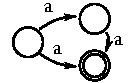
\includegraphics{img/nondeterministic_automaton.pdf}
  \caption{Beispiel eines nicht-deterministischen Automaten}
  \label{fig:nondeterministic_automaton}
 \end{center}
\end{figure}

\subsection{Konventionen und Beispiele}
%
Ich möchte hier noch auf Konventionen im Bereich der formalen Grammatiken aufmerksam machen. So ist es üblich den leeren String ,,`` mit einem $\varepsilon$ darzustellen, um Missverständnisse vorzubeugen und ihn als druckbares Zeichen darzustellen.

Wendet man reguläre Ausdrücke in Programmiersprachen an, entdeckt man, dass Ausdrücke auf Teile des Gesamtwortes angewendet werden und nicht den gesamten String matchen müssen. Hierfür existieren die Operatoren \^{} und \$, welche den Anfang und das Ende eines Strings repräsentieren. Jenes Zeichen welches einem \$ vorangestellt ist, muss also das letzte Zeichen des Eingabestrings sein. Die Verwendung dieser Operatoren ist im sprachtheoretischen Kontext nicht notwendig, da stets davon ausgegangen wird, dass der gesamte String gematcht werden soll.

In Tabelle~\ref{tab:regex_examples} sind Beispiele für reguläre Ausdrücke dargestellt.
\index{Reguläre Ausdrücke!Beispiel}
%
\begin{table}[p]
 \begin{center}
  \begin{tabular}{ll}
    \hline \hline
      \emph{matcht} & \emph{matcht nicht} \\
    \hline \hline
      \multicolumn{2}{c}{\texttt{(ab)?|cd}} \\
    \hline
      $\varepsilon$ & abcd \\
      ab & abab \\
      cd & \\
    \hline
      \multicolumn{2}{c}{\texttt{(ab|cd)*}} \\
    \hline
      $\varepsilon$ & a \\
      abcd & d \\
      abab & abc \\
      cd & \\
    \hline
      \multicolumn{2}{c}{\texttt{a?a+}} \\
    \hline
      a & $\varepsilon$ \\
      aa & b \\
      aaa & \\
    \hline
      \multicolumn{2}{c}{\texttt{(a(b|c)+d|e?)+}} \\
    \hline
      $\varepsilon$ & ad \\
      acd & ea \\
      abcd & d \\
      acccde & \\
      eabbde & \\
    \hline
      \multicolumn{2}{c}{\texttt{a?b*c+}} \\
    \hline
      abc & a \\
      ac & ab \\
      c & aabc \\
      bbbc & \\
    \hline
      \multicolumn{2}{c}{\texttt{(a?b?b)*a?}} \\
    \hline
      ab & aa \\
      abbb & baaba \\
      ababbabbba & bbbaaa \\
    \hline
      \multicolumn{2}{c}{\texttt{(ab+a*)+ab+}} \\
    \hline
      abab & aba \\
      abbbab & abb \\
      abbbaaabbbab & abbaaaba \\
      abaabbb & abbbaaba \\
    \hline \hline
  \end{tabular}
  \caption{Beispiele für reguläre Ausdrücke und deren Matching-Verhalten}
  \label{tab:regex_examples}
 \end{center}
\end{table}

\begin{figure}[p]
 \begin{center}
  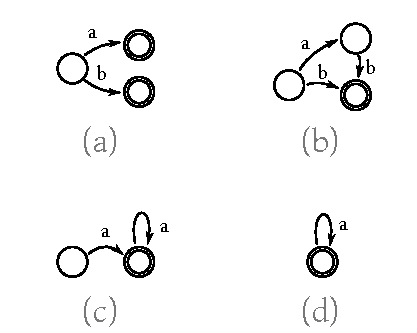
\includegraphics{img/basic_deterministic_automatons.pdf}
  \caption{
    Die deterministischen Automaten der Sprachen
    (a) \gramm{a|b} (b) \gramm{a?b} (c) \gramm{a+} (d) \gramm{a*}
  }
  \label{fig:basic_automatons}
 \end{center}
 \begin{center}
  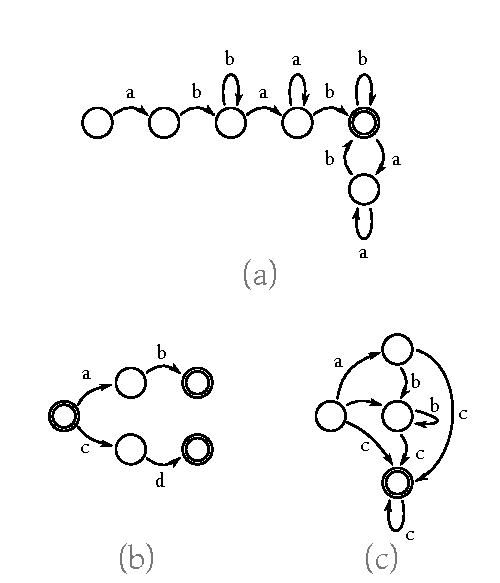
\includegraphics{img/deterministic_automatons.pdf}
  \caption{Die deterministischen Automaten der Sprachen
    (a) \gramm{(ab+a*)+ab+} (b) \gramm{(ab)?|cd} (c) \gramm{a?b*c+}}
  \label{fig:example_automatons}
 \end{center}
\end{figure}

\section{Kontextfreie Sprachen}
\index{CFL}
\index{Kontextfreie Sprache}
%
Kontextfreie Sprachen (engl. ,,context-free languages``) sind mächtiger als reguläre Sprachen. Diese Behauptung besagt, dass die Menge der Sprachen die durch reguläre Ausdrücke repräsentiert werden können kleiner als die Menge der Sprachen ist, die mit kontextfreien Sprachen spezifiziert werden können. Wir betrachten ein Beispiel.

Gesucht sei folgende Sprache $E$:
\begin{quote}
  Die Anzahl von ,,a`` ist gleich der Anzahl von ,,b``. 
\end{quote}

Probieren wir einen regulären Ausdruck zu finden.
\lstset{language={}, label={lst:cfg_regex1}, caption={Regulärer Ausdruck für die Sprache $E$}, frame={single}}
\begin{lstlisting}
(ab)*
\end{lstlisting}

Die formale Grammatik für $E$ sieht folgendermaßen aus:
\lstset{language={}, label={lst:regex_A}, caption={Sprache $E$ als formale Grammatik}, frame={single}, escapechar=\@}
\begin{lstlisting}
S @$\rightarrow$@ abS
S @$\rightarrow$@
\end{lstlisting}

Bisher war jedoch die Reihenfolge der Zeichen undefiniert. Wir erweitern nun $E$ zur Sprache $F$:
\begin{quote}
  Eine Sequenz von ,,a`` wird von einer Sequenz der gleichen Länge von ,,b`` gefolgt.
\end{quote}
In Mengennotation wäre dies mit $\set{a^n b^n \mid n \in \mathbb{N}, n \geq 0}$ anzugeben.

Durch die Vorgabe der Position bekommen wir ein neues Problem. Wir versuchen es mit folgendem regulären Ausdruck:
\lstset{language={}, label={lst:rep}, caption={Versuch eines regulären Ausdrucks für die Sprache $F$}, frame={single}}
\begin{lstlisting}
a*b*
\end{lstlisting}

Das geübte Auge erkennt, dass die Anzahl der erzeugten ,,a`` ungleich der Anzahl von ,,b`` sein kann. Daher repräsentiert dieser reguläre Ausdruck nicht die spezifizierte Sprache. So ist etwa ,,aaab`` in der Sprache des regulären Ausdrucks enthalten, aber nicht in der textuellen Beschreibung. Wir erkennen, dass die vorliegende Sprache sich nicht mehr regulär abbilden lässt, sondern ,,kontextfrei`` ist. Es handelt sich um unsere erste Sprache, die in der Menge der kontextfreien Sprachen aber nicht in der Menge der regulären Sprachen liegt.

\index{Kontextfreie Sprache!Beispiel}
Mithilfe einer formalen Grammatik können wir diese Sprache jedoch definieren:
\lstset{language={}, label={lst:lang_F}, caption={Formale Grammatik für Sprache $F$}, frame={single}, escapechar=\@}
\begin{lstlisting}
S @$\rightarrow$@ aSb
S @$\rightarrow$@
\end{lstlisting}

Basierend auf S können wir jetzt beliebige Wörter der Sprache ableiten. So nehmen wir etwa $n=3$ an:
\[
  \text{S} \rightarrow \text{aSb} \rightarrow \text{aaSbb} \rightarrow
  \text{aaaSbbb} \rightarrow \text{aaaSbbb} \rightarrow \text{aaabbb}
\]

Für kontextfreie Grammatiken dürfen wir Nonterminale definieren, die ersetzt werden. Die Idee für diese Grammatik ist es bei jeder Rekursion auf der linken und rechten Seite der Rekursion Zeichen zum endgültigen String hinzuzufügen.

Wir müssen dabei beachten, dass wir auf der linken Seite nur ein Nonterminal verwenden dürfen, um wirklich eine kontextfreie Sprache zu spezifizieren.

\section{Kontext-sensitive Sprache}
\index{Kontext-sensitive Sprache}
%
Eine weitere Menge stellen die kontext-sensitiven Sprachen dar. Dazu sei folgende Sprache zu formulieren:
\[
  H = \set{a^n b^n c^n \mid n \in \mathbb{N}, n \geq 0}
\]

\index{Kontext-sensitive Sprache!Beispiel}
Wir setzen wieder eine Grammatik an und versuchen durch Gegenbeispiele ihre Falschheit zu zeigen.
\lstset{language={}, label={lst:cflcsl}, caption={Lösungsversuch für Sprache $H$}, frame={single}, escapechar=\@}
\begin{lstlisting}
S @$\rightarrow$@ aSbB
S @$\rightarrow$@
B @$\rightarrow$@ Bc
B @$\rightarrow$@
\end{lstlisting}

Die Grammatik in Listing~\ref{lst:cflcsl} ist inkorrekt. Mithilfe der Ableitung
\[
  \text{S} \rightarrow \text{aSbB} \rightarrow \text{abB} \rightarrow 
  \text{abBc} \rightarrow \text{abBcc} \rightarrow \text{abcc}
\]
können wir uns ein Wort bauen, welches aus der Grammatik aus Listing~\ref{lst:cflcsl} stammt allerdings nicht Teil der Menge $H$ ist. Daher ist die Grammatik fehlerhaft. Die Anzahl der ,,a`` und ,,b`` sind äquivalent, aber die ,,c`` sind unabhängig.

Wir müssen unsere Grammatik ausbauen und auf der linken Seite sowohl Terminale als auch Nonterminale verwenden:
\lstset{language={}, label={lst:cslsample}, caption={Die kontext-sensitive Grammatik $\set{a^n b^n c^n \,|\, n \in \mathbb{N}_0}$}, frame={single}, escapechar=\@}
\begin{lstlisting}
S @$\rightarrow$@ aSBC
S @$\rightarrow$@
aB @$\rightarrow$@ ab
bB @$\rightarrow$@ bb
bC @$\rightarrow$@ bc
CB @$\rightarrow$@ BC
bC @$\rightarrow$@ bc
cC @$\rightarrow$@ cc
\end{lstlisting}

Zum ersten Mal verwenden wir ein Terminalsymbol und ein Nonterminalsymbol oder 2 Nonterminalsymbole zugleich auf der linken Seite. Dies ist erst bei kontext-sensitiven Sprachen erlaubt.

\section{Chomsky-Hierarchie}
\index{Chomsky-Hierarchie}
%
Wir haben bei diesen Beispielen gesehen, dass gewisse Modelle nicht ausreichen, um Sprachen zu beschreiben. Noam Chomsky hat die Chomsky-Hierarchie formuliert, um Sprachen in Kategorien einzuteilen. Dabei sind reguläre Sprachen die schwächsten Sprachen. Kontextfreie Sprachen stehen über den regulären Sprachen und können auch alle regulären Sprachen abbilden. Am mächtigsten sind die rekursiv-aufzählbaren Sprachen, die es etwa erlauben die Anzahl der Rekursionen in den Ersetzungsregeln während der Verarbeitung zu verändern. Wir möchten hier auf weitere Beispiele verzichten und auf die Lehrveranstaltung \courseswp{} verweisen, welche sich detailierter mit diesen Sprachen auseinander setzt.

Abbildung~\ref{fig:chomsky_hierarchy} visualisiert die Chomsky-Hierarchie.
%
\begin{figure}[h]
 \begin{center}
  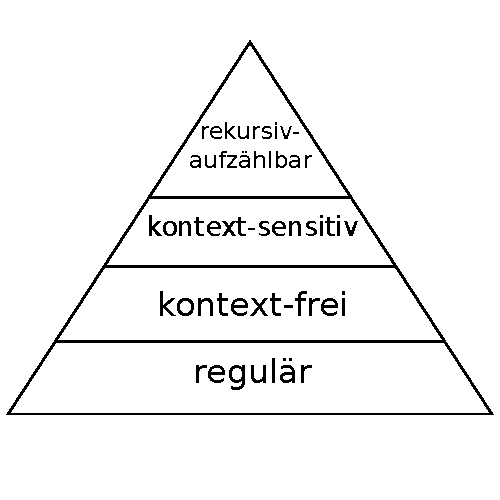
\includegraphics{img/chomsky_hierarchy.pdf}
  \caption{Die Chomsky-Hierarchie}
  \label{fig:chomsky_hierarchy}
 \end{center}
\end{figure}
